\documentclass{final-report}

\title{You can solve it, but can you play it?}

\subtitle{Puzzles, games, and the polynomial hierarchy}

\author{Kye Shi}
\advisor{Nicholas Pippenger}
\reader{Arthur T. Benjamin}
\date{2021 November}

\bibliography{bibliography.bib}
\bibliography{newbib.bib}

\definecolor{ks0}{HTML}{0050c0}
\definecolor{ks1}{HTML}{e00060}
\definecolor{ks2}{HTML}{f0b000}

\tikzset{
  gates/.style={
    row sep=1em/2,
    column sep=2em,
    matrix of nodes,
  },
  every circuit symbol/.style={
    fill,
    fill opacity=1/8,
    anchor=output,
  },
  vertex/.style={
    circle,
    draw,
    minimum size=1em/2,
    inner sep=0pt,
  },
  vertex label/.style={
    text height=2em/3,
    text depth=1em/3,
  },
  edge/.style={
  },
  wire/.style={
    rounded corners=1em/4,
    to path={
      -- ($ (\tikztostart)!1em!(\tikztostart -| \tikztotarget) $)
      -- ($ (\tikztotarget)!1em!(\tikztostart |- \tikztotarget) $)
      -- (\tikztotarget)
    },
  },
}

\begin{document}

\frontmatter
\maketitle
\tableofcontents

draft outline:

\begin{itemize}
  \item Introduction and overview.
  \item Basic complexity background: P, reductions, completeness
  \item More complexity background---NP, PSPACE, polynomial hierarchy as games,
    etc. Haven't made up my mind yet about whether to introduce this abstractly
    on its own, or introduce it concurrently with CSAT games to keep things
    concrete/tangible.  I'm leaning the latter.
    \begin{itemize}
      \item Circuit value, satisfiability games
    \end{itemize}
  \item SAT variation games
    \begin{itemize}
      \item Circuits could just as well be plain boolean formulae, or CNF
        formulae, etc.; list some prior work on other known SAT games in
        PSPACE, polynomial-hierarchy, etc.  (paper on this in ann. bib.)
    \end{itemize}
  \item Graph coloring games
    \begin{itemize}
      \item Intro---overview of existing results: NP-completeness of graph
        coloring, col and snort as PSPACE-complete games.
      \item Custom presentation of NP-completeness proof via circuit reduction
      \item Introduction of 2-turn game, 3-turn game, k-turn game, etc.
      \item Complexity claims and proofs
    \end{itemize}
  \item Exact-covering games
  \item three-dimensional matching games
  \item Conclusion % only a few of countlessly many problems introduced/explored
\end{itemize}


\mainmatter

\chapter{Introduction}

The basic question of computational complexity---``how hard is this problem for
a computer to solve?''---is central to nearly every topic in computer science.
And yet the formalisms of complexity theory often seem, in my own experience,
intimidatingly abstract, phrased in terms of intangible models of computation
such as non-deterministic Turing machines and oracles.

The remedy, I believe, lies in studying complexity theory through the lens of
\emph{puzzles} and \emph{games}.  Not only do they provide a concrete grounding
for the abstractions, they also offer a particularly insightful, accessible,
and most importantly fun approach to understanding complexity theory.  In fact,
many of the most popularly known and appreciated results in complexity theory
are those about so-called ``\NP-complete puzzles'', such as Sudoku, and
``\PSPACE-complete games'', such as Checkers and Go.

This thesis emphasizes that approach in its exploration of a particularly
foundational, yet often overlooked, ladder of complexity classes known as the
\emph{polynomial hierarchy}.  \NP{} is the class of (one-player) ``puzzles'',
and \PSPACE{} is the class of (two-player) ``games'' of polynomial length; the
polynomial hierarchy, then, lies in the middle, encompassing games of
\emph{fixed} length.  Through this lens, the (in)famous \P-vs-\NP{} question is
but the first in a ladder of questions that are, arguably, just as crucial and
impactful.

%The polynomial hierarchy is as central to
%complexity theory as the \P-vs-\NP{} problem is well-known.

\section{Overview}

This document is structured as follows.  First, \cref{ch:background,ch:boolean}
establish preliminary background concepts and conventions adopted throughout
this thesis.  Next, \cref{ch:circuit} lays the central theoretical groundwork,
defining the \emph{polynomial hierarchy} through a fundamental family of
problems known as the \Problem{Circuit Satisfiability} games.  Next,
\cref{ch:misc} explores a novel family of games generalized from the
\Problem{Graph 3-Colorability} puzzle and establishes \emph{hardness} bounds on
each of those games.  Finally, \cref{ch:conclusion} concludes by discussing the
future directions of this work and its broader implications.

\section{Prior work and inspirations}

Much of the background exposition on complexity theory referenced in this thesis
is reproduced from Christos Papadimitriou's textbook,
\citet{papadimitriou.cc} (though many of the foundational ideas were
originally introduced/proven elsewhere, e.g.
\citet{cook.np,levin.np,stockmeyer.ph}), reframed through the
puzzles-and-games perspective and supplemented with a few comments on intuition.

The main family of games explored in this thesis, fixed-turn
\Problem{3-Colorability} games (\cref{ch:misc}), is a generalization of
(one-turn) \Problem{3-Colorability}, a well-known \NP-complete puzzle originally
proven \NP-complete by \citet{karp.np}.  Others have studied (multi-turn)
game generalizations of \Problem{3-Colorability}, but all versions that I've
encountered are \PSPACE-complete, in which the number of turns played during the
game scales proportionally with the size of the graph
\citep{bodlaender.coloring,bh.placement,kbd.impartial,cpss.coloring,schaefer.games}. As far as I'm aware, the variations I explore here—with fixed
numbers of turns regardless of the size of the graph—is unexplored, and the main
theorem about its \SigmaP k-completeness (\cref{th:yayay}) is novel.  The basic
idea underlying my proof is the composition of two well-known results:
\begin{itemize}[nosep]
  \item \citet{karp.np}'s classic proof of the \NP-hardness of the \Problem{3-Colorability} puzzle, via a reduction from \Problem{3CNF-Satisfiability};
  \item 's transformation from boolean circuits to equivalent 3CNF-clauses.
\end{itemize}

Without further ado, let's begin.


%TODO: outline/overview of chapters, after those chapters are written

%TODO: also give general citations here, e.g. papadimitriou for many
%foundational background info, etc.
%
%TODO: notation table also belongs in this chapter i think

%p-vs-np well known, polynomial-hierarchy central

%puzzles and games; hierarchy lies in the interstices.  we examine a few
%interesting (by no means exhaustive, or even close to comprehensive)
%np-complete puzzles with pspace-complete analogues, and we









%Famously central to the theory of computational complexity is the \P-vs-\NP{}
%question, and essential to our understanding of that question is the study of
%\NP-complete problems such as the Boolean Satisfiability puzzle, the Graph
%Colorability puzzle, and countless more.  Puzzles like these, which nearly any
%layperson can appreciate, offer a particularly insightful, intuitive, and
%\emph{fun} lens through which to study computational complexity. Explorations
%of more complex problem-classes such as \PSPACE{} can be similarly approached
%through the study of strategic decision \emph{games} such as Othello, Checkers,
%and Go.
%
%What lies in the interstices between \emph{puzzles} and \emph{games}?  How do
%we take a puzzle and generalize it into a game, and what are the puzzle-games
%we encounter along the way?  And how hard exactly are these puzzle-games to
%decide?  These questions are the focus of my thesis.

%So far, I have explored these questions from three angles:
%\begin{enumerate}
%
%  \item \label{itm:intro.q.generation} Puzzle generation.  If I wish to solve a
%    puzzle, you can play a game with me by constructing puzzle \emph{instances}
%    for me to solve.  For instance, \emph{solving} Sudoku is an \NP-complete
%    problem; your task is to \emph{generate} (partially-filled) Sudoku boards
%    for me to solve.
%
%    How hard is it to do so?  Moreover, how hard is it to generate \emph{good}
%    puzzle instances, for various definitions of \emph{good} (sufficiently
%    challenging to solve, or having unique solutions, or solvable/unsolvable by
%    certain strategies)?
%
%    % lauren sanchis
%
%  \item \label{itm:intro.q.pspace} \PSPACE-complete games derived from
%    \NP-complete puzzles.  A canonical \NP-complete puzzle is the \Problem{sat}
%    (Boolean Satisfiability) puzzle: given a Boolean formula \(\phi(x_1, \dots,
%    x_n)\), does there exist an assignment to its inputs \(x_1, \dots, x_n\)
%    such that \(\phi(\dots) = 1\)? In an analogous game, two players alternate
%    turns assigning \(x_1, \dots, x_n\); player 1 wins if \(\phi(\dots)=1\),
%    and player 2 wins if \(\phi(\dots)=0\).  Does either player have a
%    (guaranteed) winning strategy?  This game, known as \Problem{qsat}
%    (Quantified Satisfiability), is a canonical example of a \PSPACE-complete
%    game.
%
%    Can other \NP-complete puzzles be similarly generalized into games?  Will
%    those games also be \PSPACE-complete?
%
%    % schaefer
%
%  \item \label{itm:intro.q.ph} Fixed-turn games and the polynomial hierarchy.
%    In between the complexity classes \NP{} and \PSPACE{} lies a chain of
%    increasingly-complex problem-classes known as the \emph{polynomial
%    hierarchy}.  In some cases, problems in the polynomial hierarchy may be
%    thought of as game generalizations of \NP-complete puzzles with a
%    \emph{fixed} number of turns.  For instance, in a two-turn version of
%    \Problem{sat}, inputs are partitioned into two (disjoint) groups \(X_1\)
%    and \(X_2\); on turn 1, player 1 assigns \(X_1\), and on turn 2, player 2
%    assigns \(X_2\).  As before, player 1 (respectively 2) wins if
%    \(\phi(\dots) = 1\) (respectively \(0\)).  Determining whether player 1 has
%    a winning strategy is complete for a complexity class known as
%    \(\SigmaP2\), which lies just above \NP{} in the hierarchy, and analogous
%    games with \(k\) turns are \(\SigmaP k\)-complete.
%
%    Do polynomial-hierarchy generalizations of other \NP-complete puzzles
%    exist?
%
%\end{enumerate}
%
%\Cref{ch:progress} discusses my progress so far in each of these areas.
%Questions \ref{itm:intro.q.generation} and \ref{itm:intro.q.pspace} have been
%explored in-depth by others, while question \ref{itm:intro.q.ph} appears to be
%scarcely explored.  As such, I provide only brief summaries of/reflections on
%the existing work pertaining to \ref{itm:intro.q.generation} and
%\ref{itm:intro.q.pspace}.  Meanwhile, I describe in greater detail question
%\ref{itm:intro.q.ph}, which is the focus of my explorations so far.
%
%\Cref{ch:future} summarizes the primary questions \& goals that will guide
%my exploration next semester.
%
%Finally, \cref{ch:bib} contains an annotated bibliography of existing work
%pertaining to each of these topics.



\chapter{Basic concepts in complexity theory}

The fundamental question driving the study of computational complexity theory
is, ``how difficult are certain problems for computers to solve?''  In order to
answer this question precisely, we must start by figuring out what exactly it
asks.  That is, formally, what do we mean by \emph{difficulty}?  For that
matter, what constitutes a \emph{problem}?  What counts as a \emph{computer}?

Conventionally, \emph{computers} are formalized as Turing machines, with
\emph{difficulty} being measured by the number of Turing machine execution
steps.  For the purposes of this thesis, we avoid delving into the formalism of
Turing machines.  Instead, we assume an informal notion of computers given by
any algorithm or procedure straightforwardly implementable in modern,
high-level programming languages such as C/C++, Python, Java, etc.  Detailed
treatment of the relevant formalisms may be found in \textcite[Chapter
2]{papadimitriou.cc}.  In particular, there are theorems \parencite[Theorem
2.5]{papadimitriou.cc} showing that modern CPU/RAM-based computer architectures
are, for our purposes, equivalent to Turing machines, thereby justifying the
informal approach we take here.

In the following sections, we discuss what exactly constitutes a
\emph{problem}, how we describe the complexity (i.e., difficulty) of problems,
and how we categorize problems by difficulty into \emph{complexity classes}.

%emphasize intuitive descriptions of
%algorithms in terms of modern, ``high-level'' programming concepts exhibited by
%programming languages such as Python.

%An
%alternative treatment uses ``random access machines'', which mimic modern
%CPU/RAM-based computer architectures.  In this thesis, we avoid delving into
%these formal details.

%in terms of modern, high-level programming concepts

%In the conventional formalism, computers are modeled as Turing machines.
%Difficulty, then, refers to the number of execution steps required by a Turing
%Machine to solve a problem.  Alternatively, computers could be modeled as
%``random access machines'' \parencite[Section 2.6]{papadimitriou.cc}, which
%mimic modern CPU/RAM-based computer architectures.  For our purposes, the two
%models of computation are equivalent \parencite[Theorem 2.5]{papadimitriou.cc}.

%Formal treatments of these
%definitions are found in \textcite[Chapter 2]{papadimitriou.cc}

%Of particular
%note, \textcite[Theorem 2.5]{papadimitriou.cc} shows that these two models of
%computation are, for our purposes, equivalent.  Therefore, for our purposes, we will
%assume the latter model, allowing us to think in terms of modern programming
%patterns and give

%By \emph{hardness}, what we really mean is: given a problem input
%encoded in \(n\) bits, how much computational time, asymptotically with respect
%to \(n\), is required to solve that problem?  In order to discuss this question
%precisely, we have to clearly define what we mean by ``computational time'',
%and, for that matter, what we mean by ``computer''.  A traditional approach
%takes ``computer'' to mean Turing Machines and ``time'' to be Turing Machine
%execution steps; another approach defines ``computer'' via modern-day,
%CPU/RAM-based architectures, with ``time'' given by CPU instruction cycles.

%relatively \emph{informal} descriptions of algorithms.

\section{Decision problems}

The simplest flavor of computational problem is a \emph{decision problem}, or a
yes/no question: given an input \(X\), does \(X\) satisfy certain conditions?
Here are some examples of decision problems:
\begin{itemize}[nosep]
  \item Given an integer \(K\), is \(K\) even?
  \item Given a string of letters \(S\), is \(S\) a palindrome?
  \item A silly decision problem, but nevertheless a valid one: given any input
    \(X\), always return ``yes''.
\end{itemize}

In order for a yes/no question to qualify as a decision problem, it must be
stated in terms of an arbitrary input.  For instance, consider the following
question:
\begin{itemize}[nosep]
  \item Is \(314159\) a prime number?
\end{itemize}
This is a yes/no question, but it takes no inputs (the value \(314159\) is not
an input; it is merely part of the question statement).  In this sense, it is
computationally uninteresting: in order to solve this question, an algorithm
only needs to return the fixed answer ``yes''.  In contrast, what we're really
interested in is the general problem of primality testing:
\begin{itemize}[nosep]
  \item Given an arbitrary positive integer \(K\), is \(K\) prime?
\end{itemize}

We formalize the definition of decision problems below.

\begin{definition}{(decision) problem}{}

  A \Term{decision problem} is a function
  \(Π\colon\Set{0,1}^*→\Set{\text{yes},\text{no}}\).  Equivalently, a
  \Term{decision problem} is the set \(Π⊆\Set{0,1}^*\) comprising exactly the
  inputs, a.k.a. \Term{instances}, that result in ``yes'' answers.

  That is, for any input \(X∈\Set{0,1}^*\), we say \(X∈Π\) (in the \emph{set}
  sense) if \(Π(X)=\text{yes}\) (in the \emph{function} sense), and \(X∉Π\) to
  mean \(Π(X)=\text{no}\).

  \begin{aside}
    Formally, inputs to decision problems are always encoded as binary strings.
    Essentially, this requirement follows from the fact that all modern
    computers encode data in binary anyway.  Furthermore, it allows us to
    rigorously discuss notions such as \emph{input size}.  This is an important
    formal detail, but for the most part, we avoid dealing with any binary
    encoding/decoding technicalities.  We mention this detail here only to
    clarify the role of \(\Set{0,1}^*\) in the definition above.
  \end{aside}

\end{definition}

A more general notion of \emph{problems} considers arbitrary (binary-encoded)
functions \(\Set{0,1}^*→\Set{0,1}^*\); this notion is termed \Term{function
problems}.  However, we will focus mainly on decision problems for two reasons.
First, decision problems are easier to work with than function problems.
Second, function problems can be encoded in terms of decision problems (e.g.,
mapping each output bit to its own decision problem).  Essentially, the
\emph{decision problem} formalism is conceptually simpler but remains versatile
enough to capture the important core ideas of complexity theory. As such, the
vast majority of the problems examined in this thesis are decision problems.
For convenience we will simply say ``problems'' to mean decision problems,
unless otherwise specified.

\section{Complexities and classes}

When we ask how difficult a problem is, we are essentially asking, how much
time (or other resources, such as memory) does a computer need to solve that
problem?  Of course, the answer depends on the input: some inputs are easy to
solve, and others are harder.  Certainly, we expect the difficulty to scale
with input size: the larger the input, the more work it generally takes an
algorithm to process it.  Thus, the complexity of a problem is given as a
function of the input size.  Specifically, we ask, if an algorithm is given an
input string (recall, encoded in binary) of length \(n\), how much time in the
worst case is required, as a function of \(n\)?

However, exact function bounds are unnecessarily sensitive to pedantic
technicalities, e.g., slight variations in implementations of the same
algorithm, or specific details in the formal models of ``computer''. Instead,
loosely speaking, we are mostly interested in how these costs asymptotically
\emph{scale} as the input size gets large.  Thus, we categorize problems with
``similar'' complexities into \emph{complexity classes}.

So then, what counts as \emph{similar}?  As a starting approximation, we assert
that \emph{polynomials are small}: any algorithm whose running time is bounded
by some polynomial function is considered relatively ``fast''; problems with
polynomial-time solutions are considered relatively ``easy''.  We formalize
this idea in the definition of the complexity class \P{} below.

\begin{definition}{Polynomial-time problems, \P}{}

  Let \(A\) be an algorithm computing some (decision) problem (i.e., it takes a
  binary string as input and returns ``yes'' or ``no'').  We say \(A\) runs in
  \Term{polynomial time} if there exists some polynomial \(p\) such that, on
  any input \(X∈\Set{0,1}^*\), the algorithm \(A\) terminates in \(≤p(\Abs X)\)
  steps.

  The complexity class \P{} is the set of (decision) problems correctly
  solvable in polynomial time.

  \begin{aside}
    For contrast, we say an algorithm is \Term{super-polynomial} if its running
    time cannot be bounded by some polynomial.  Examples of super-polynomial
    functions include \(n^{\log n}\), \(2ⁿ\), etc.
  \end{aside}

\end{definition}

To be clear, taking polynomials to mean ``easy'' is a very crude rule-of-thumb:
there are important practical subdivisions \emph{within} \P{} that this
categorization plainly ignores (e.g., linear-time vs quadratic-time); there are
also a few notable examples of super-polynomial-time algorithms that are, by
this rule, slow, but quite efficient \emph{in practice} (e.g., the simplex
algorithm for linear programming).  Nevertheless, this delineation remains an
extremely useful (and arguably elegant) starting point for the classification
of problems.

% TODO examples of 𝐏 problems, and perhaps discuss papadimitriou theorem 2.5
% again with more precision?

\section{Hard problems and reductions}

Above, we establish that a problem is considered \emph{easy} if it has a
polynomial-time solution.  Hard problems, then, are those without
polynomial-time solutions… right?  Sure.  But how do we go about showing that a
problem is actually hard?  And how hard, exactly?

For an easy problem, proving \emph{existence} of a polynomial-time algorithm is
straightforward---simply construct one.  On the other hand, for a problem that
appears to be hard, we would have to prove \emph{non-existence} of a
polynomial-time algorithm---that it is \emph{impossible} to find a
polynomial-time algorithm. In general, this is incredibly difficult to show;
this difficulty is largely why the infamous \P-vs-\NP{} question remains
unsolved.

Instead, we take a different approach to understanding hard problems: comparing
them to each other.  To illustrate, consider the following two problems:

\begin{description}

\item[\Problem{Latin Square}] Given a square grid of dimensions \(n×n\) (for
  some \(n\)), with some of its cells filled in with a number in
  \(\Set{1,\dotsc,n}\), is it possible to complete the remaining cells so that
  each row and each column contains each number exactly once?

  \begin{figure}[H]
    \begin{center}
      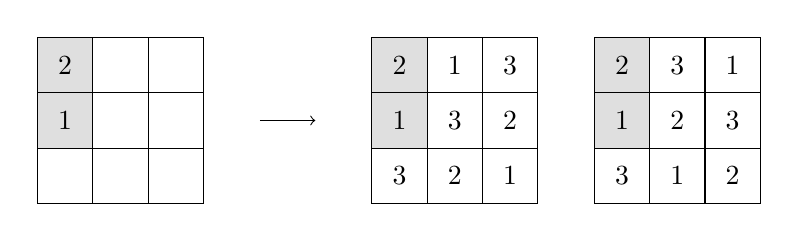
\begin{tikzpicture}[x=2em, y=2em]

        \tikzset{
          ls/.pic={
            \draw
            (0,0) rectangle (3,3)
            foreach \i in {1,2} { (0,\i) -- +(3,0) (\i,0) -- +(0,3) };

            \foreach \i/\j/\n in {0/2/2,0/1/1} {
              \fill[opacity=1/8] (\i,\j) rectangle +(1,1);
              \node at (\i+1/2,\j+1/2) {\(\n\)};
            };
          },
          lss/.pic={
            \pic{ls};
            \node at (1/2,1/2) {\(3\)};
            \foreach \i in {0,1,2} {
              \pgfmathtruncatemacro\m{Mod(\i+#1-1,3)+1}
              \pgfmathtruncatemacro\n{Mod(\i-#1-1,3)+1}
              \node at (1+1/2,\i+1/2) {\(\m\)};
              \node at (2+1/2,\i+1/2) {\(\n\)};
            }
          },
        }

        \matrix[column sep=2em] {
          \pic{ls}; & \draw[->] (0,3/2) -- +(1,0); &
          \pic{lss=-1}; & \pic{lss=1}; \\
        };

      \end{tikzpicture}

      \caption{A \(3×3\) Latin Square instance and its two possible
      completions.}

      \label{fig:background.latin-square-example}

    \end{center}
  \end{figure}

\item[\Problem{Graph Coloring}] Given a positive integer \(k\), and a graph
  with \(n>k\) vertices, some of which are assigned a number (a.k.a. ``color'')
  in \(\Set{1,\dotsc,k}\), is it possible to assign numbers to the remaining
  cells so that no neighboring vertices receive the same assignment?

  \begin{figure}[H]
    \begin{center}
      \begin{tikzpicture}


      \end{tikzpicture}
    \end{center}
  \end{figure}


  TODO diagram illustrations.  also i wish i could think of simpler-to-state
  examples with easy reductions, but nothing comes to mind, so this is the best
  i've got for now.

\end{description}

Is one of these problems ``easier'' than the other?  In a sense, yes: the
\Problem{Latin Square} problem is just a special case of the \Problem{Graph
Coloring} problem, where the vertices are arranged into a square grid, and all
vertices in the same row or column neighbor each other.

\begin{figure}[H]
  \begin{center}
    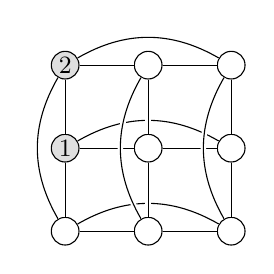
\begin{tikzpicture}[x=3em, y=3em]

      \tikzset{
        vert/.style={circle, draw, minimum size=1em, inner sep=0pt, font=\small},
        pre/.style={vert, fill, fill opacity=1/8, text opacity=1},
        edge/.style={preaction={draw=white, line width=2pt}},
      }

      \node[pre](02) at (0,2) {\(2\)};
      \node[pre](01) at (0,1) {\(1\)};
      \coordinate[vert](00) at (0,0){};

      \foreach \i in {1,2} { \foreach \j in {0,1,2} {
          \coordinate[vert](\i\j) at (\i,\j);
      } };

      \draw[edge] foreach \i in {0,1,2} { (0\i) to[bend left] (2\i) };
      \draw[edge] foreach \i in {0,1,2} { (\i0)--(\i1)--(\i2) (0\i)--(1\i)--(2\i) };
      \draw[edge] foreach \i in {0,1,2} { (\i0) to[bend left] (\i2) };

    \end{tikzpicture}

    \caption{The Latin Square from \cref{fig:background.latin-square-example},
    represented as a graph.}

  \end{center}
\end{figure}

More precisely, this argument describes a way to convert any \Problem{Latin
Square} instance (a partially-filled \(n×n\) grid) into a \Problem{Graph
Coloring} instance (a partially-colored graph with \(n²\) vertices) with the
same yes/no answer.  Formally, we call this conversion a \Term{reduction}:

\begin{definition}{reductions}{}

  Let \(Π₁\) and \(Π₂\) be decision problems.  A \Term{reduction} from \(Π₁\)
  to \(Π₂\) is an algorithm \(R\colon\Set{0,1}^*→\Set{0,1}^*\) such that, for
  each \(X∈\Set{0,1}^*\), \(X∈Π₁\) if and only if \(R(X)∈Π₂\).

  In other words, \(R\) converts problem-inputs (a.k.a. \emph{instances}) of
  \(Π₁\) to problems-inputs of \(Π₂\) such that the yes/no answers on the
  original and converted inputs exactly match.

  %\begin{aside}
  %  %This definition is sometimes called \emph{Karp reductions} or
  %  %\emph{many-one reductions}, in order to distinguish it from other notions
  %  %of reduction such as \emph{Turing/Cook reductions} and \emph{truth-table
  %  %reductions}, which are related but different.

  %  %For our purposes, Karp reductions are the simplest to describe and
  %\end{aside}

\end{definition}

Revisiting the above example, the existence of a reduction from \Problem{Latin
Square} to \Problem{Graph Coloring} captures the idea that \Problem{Latin
Square} is easier than \Problem{Graph Coloring} in the following sense.
Suppose that we already know how to solve \Problem{Graph Coloring}.  Then, we
automatically also know how to solve \Problem{Latin Square}: given an arbitrary
\Problem{Latin Square} input, apply the reduction to convert it into a
\Problem{Graph Coloring} input, feed that input into the known \Problem{Graph
Coloring} solver, then directly return its answer.

However, in order to authentically capture the idea of \emph{easiness}, we must
also account for computation time.  Namely, we stipulate that the reduction
itself must be efficient---formally, that it runs in polynomial time.

\begin{definition}{polynomial-time reducibility}{}

  Let \(Π₁\) and \(Π₂\) be decision problems.  We say \(Π₁\) is
  \Term{polynomial-time-reducible} to \(Π₂\), which we denote as
  \[
    Π₁≤Π₂,
  \]
  if there exists a reduction from \(Π₁\) to \(Π₂\) that runs in polynomial
  time.  (The \(≤\) notation evokes the intuition that \(Π₁\) is easier than,
  or \emph{at most as hard as}, \(Π₂\).)

\end{definition}

Finally, we introduce some terminology to describe how one problem compares to
a \emph{class} of problems:

\begin{definition}{hardness and completeness}{}

  Let \(Π\) be a decision problem, and let \(\C\) be a class of decision
  problems.

  We say \(Π\) is \Term{hard} for \(\C\), or \Term{\C-hard}, if every
  problem in \C{} is polynomial-time-reducible to \(Π\).

  We say \(Π\) is \Term{complete} for \C, or \Term{\C-complete}, if \(Π\) is
  \C-hard and \(Π∈\C\).

  \begin{aside}
    Following the intuition that reducibility (\(≤\)) defines a (partial)
    ordering of problems by difficulty, \C-hard problems are just those that
    are (non-strictly) harder than all problems in \C, and \C-complete problems
    are just the \emph{maximal/hardest} problems within \C.
  \end{aside}

\end{definition}

Complete problems are especially useful, first and foremost, because they are
tangible.  They have accessible, interesting, and often real-world-applicable
examples that help us understand complexity classes in concrete, intuitive
terms, rather than pure abstractions.  At the same time, complete problems are
also very general.  As \emph{tight} difficulty upper bounds of a complexity
class, they are perfect characterizations of these classes; determining the
exact difficulty of a complete problem automatically essentially determines the
difficulty of the entire complexity class.

%By studying complete problems for a spectrum of complexity classes, we gain
%wholesale but vivid insight

% TODO i feel like i want to have a conclusion punchline here

%Now, it is time to study a collection of complete problems
%
%satisfiability games.



%\section{Puzzles, non-determinism, and \NP}

%Consider the following problem.
%\begin{itemize}
%  \item Given a graph \(Γ\) and a positive integer \(k\), does \(Γ\) contain a
%    clique of size \(k\)?
%\end{itemize}


%\section{Hard problems and completeness}

%Notationally, we say \(X\) is \emph{in} the problem \(L\), or \(X\in L\), if
%the answer is yes; otherwise, we say \(X\notin L\).
%
%An example of a decision problem is the graph reachability problem:
%\begin{definition}[\Problem{reachability}]%
%  Given a graph with \(n\) vertices \(v_1, \dots, v_n\), does there exist a
%  path connecting \(v_1\) to \(v_n\)?
%\end{definition}
%This problem may be solved using simple graph-search algorithms such as
%Breadth-First/Depth-First Search, whose asymptotic running time is \(\O(n)\)
%---that is, bounded by a linear function of \(n\).  As such, this problem is
%considered relatively ``easy'' to solve.
%
%More generally, \Problem{reachability} belongs to the class of decision
%problems known as \P:
%\begin{definition}[\P]%
%  The class of decision problems whose solution runtime is bounded by a
%  polynomial function of the input length.
%\end{definition}
%We consider problems in \P{} to be ``easy''---at least, from the standpoint of
%computational complexity.
%
%Another example of a decision problem is the Hamiltonian path problem:
%\begin{definition}[\Problem{hamiltonian-path}]%
%  \label{def:hamiltonian-path} Given a graph with \(n\) vertices, does it
%  contain a Hamiltonian path (i.e., a path that visits each vertex exactly
%  once)?
%\end{definition}
%This problem is not known to be in \P.  In fact, the best known algorithms
%solving \Problem{hamiltonian-path} are essentially brute-force guess-and-check:
%\emph{guess} a possible Hamiltonian path (e.g., by writing down some
%permutation of the vertices), then \emph{check} that it is valid (e.g., that
%each pair of adjacent vertices in the guessed path are actually connected by an
%edge in the graph).  In the worst case, if our guesses are really unlucky, we
%may have to repeat up to \(n!\) iterations, which is definitely not polynomial.
%However, setting aside the cost associated with brute-forcing guesses, note
%that individual \emph{checking} steps \emph{do} run in polynomial time.
%Problems like this, which are solvable via guess-and-check, where the ``check''
%problem is in \P, belong to a class of problems known as \NP:
%\begin{definition}[\NP]%
%  \label{def:np} A decision problem \(L\) is in \NP{} if\dots
%  \begin{nested}
%    there exists a corresponding decision problem \(L'\in\P\) (intuitively: the
%    ``check'' problem) and a polynomial \(p\) such that\dots
%    \begin{nested}
%      for all input strings \(x\)\dots
%      \begin{nested}
%        \(x \in \NP\) if and only if\dots
%        \begin{nested}
%          there exists a ``guess'' \(g\) with length \(\Abs g \le p(\Abs x)\)
%          such that \((x, g) \in L'\) (intuitively: \(g\) passes the
%          ``check'').
%        \end{nested}
%      \end{nested}
%    \end{nested}
%  \end{nested}
%
%  Note that the \(\Abs g \le p(\Abs x)\) requirement is present in order to
%  ensure that the guesses are not so obscenely long as to abuse the idea of
%  ``efficient'' checking.  This requirement is not central to understanding the
%  definition of \NP{} but is nevertheless an important technical subtlety.
%\end{definition}
%
%The infamous \P-vs-\NP{} open question asks: is \NP{} truly more difficult than
%\P?  Does there exist some problem in \NP{} that definitively cannot be solved
%within polynomial time?  I, a baby undergraduate, am not in the business of
%answering that question.
%
%As such, the best we can do to determine the difficulty of a given problem is
%to compare them to other problems, deriving a \emph{relative} ordering telling
%us which problems are easier/harder than other ones.  To this end, we must
%define what easier/harder means---intuitively, we think of a problem \(L_1\) as
%easier than another problem \(L_2\) if knowing how to solve \(L_2\)
%automatically also tells us how to solve \(L_1\), with minimal
%(polynomially-bounded) overhead.  More precisely:
%\begin{definition}[reductions]
%  \label{def:reduction}
%  Let \(L_1\) and \(L_2\) be decision problems.  We say \(L_1\) is
%  \emph{reducible to} \(L_2\), or that \(L_1\) is \emph{at least as easy as}
%  \(L_2\)'', denoted \(L_1 \le L_2\), if\dots
%  \begin{nested}
%    there exists a function \(f\), called a \emph{reduction}, converting input
%    strings for \(L_1\) to inputs for \(L_2\), such that \(f\) is computable
%    within polynomial time, and\dots
%    \begin{nested}
%      for any input \(x_1\)\dots
%      \begin{nested}
%        \(x_1 \in L_1\) if and only if \(x_2 \in L_2\).
%      \end{nested}
%    \end{nested}
%  \end{nested}
%
%  Note that this definition of reductions is slightly different than the one
%  given in \textcite{papadimitriou.cc}, whose requirement on \(f\) is that it
%  is computable in \emph{logarithmic-space} rather than polynomial-time.
%  However, for the purposes of this project, the distinction between the two is
%  unimportant.
%\end{definition}
%
%This notion of comparison also gives us a good way of comparing problems to
%entire classes:
%\begin{definition}[hardness and completeness]%
%  \label{def:hard-complete}
%  Let \(\mathbfit C\) be a complexity class.
%  \begin{itemize}[nosep]
%    \item A problem \(L\) is \emph{hard for \(\mathbfit C\)}, or
%      \emph{\(\mathbfit C\)-hard}, if \(L\ge K\) for every \(K\in\mathbfit C\).
%    \item A problem \(L\) is \emph{complete for \(\mathbfit C\)}, or
%      \emph{\(\mathbfit C\)-complete}, if \(L\) is \(\mathbfit C\)-hard
%      \emph{and} \(L\in\mathbfit C\).
%  \end{itemize}
%\end{definition}
%
%In particular, \emph{complete} problems for a class \(\mathbfit C\) are at
%least as hard as everything else in \(\mathbfit C\) and simultaneously
%themselves \emph{in} \(\mathbfit C\).  In this sense, for any complexity class,
%its complete problems are its \emph{hardest} problems, giving us an effective,
%``exact'' characterization of the class in terms of its problems.
%
%This approach to characterizing complexity classes is the driving motivation
%behind our exploration of puzzles and games.
%
%%\todo[inline]{unfinished.  formalism of turing machines, decision problems,
%%  oracles \& the definition of polynomial hierarchy, proofs of completeness of
%%  SAT \& QSAT for classes in the polynomial hierarchy.  I imagine this stuff
%%  will be needed in the final thesis; is it needed also for the midyear
%%report?}
%%
%%\begin{definition}[decision problem/language]%
%%  A \textbf{decision problem} is a yes/no question posed on binary input
%%  strings, or problem \textbf{instances}.  As such, we may think of a decision
%%  problem as a mapping
%%  \[
%%    L \colon \Set{0, 1}^* \to \Set{\text{yes}, \text{no}}.
%%  \]
%%
%%  More commonly, we associate a problem with its ``yes'' instances, the set of
%%  which is a \textbf{language}:
%%  \[
%%    L(L) = \SetBuilder* {x \in \Set{0, 1}^*} {L(x) = \text{yes}}.
%%  \]
%%  Here, for clarity, we are distinguishing notationally between \(L\) and
%%  \(L(L)\), but in general we conflate the two notions and refer to both as
%%  the problem \(L\).
%%\end{definition}
%%
%%\begin{definition}[\NP]
%%  \NP{} is the class of problems solvable by a \emph{non-deterministic} Turing
%%  machine in \emph{polynomial time}.
%%\end{definition}
%%
%%
%%
%%

\chapter{A primer on boolean logic}
\label{ch:boolean}

Mathematical logic is founded on true-or-false statements---statements such as:
\begin{itemize}[nosep]
  \item property \(A\) is \emph{true} when condition \(B\) is \emph{false},
  \item property \(X\) is \emph{true} when both condition \(Y\) and condition
    \(Z\) are \emph{true},
\end{itemize}
and so on.  Boolean logic refers to the algebra of how \emph{truthiness} and
\emph{falsiness} combine and transform under various logical operations.

It is no surprise, given the foundational role of booleans in mathematical
logic, that they also underpin all computational logic. For instance, all
modern computer architectures deal with data encoded in binary \(0\)s
(\emph{false}) and \(1\)s (\emph{true}).  Furthermore, it follows that
everything we conceive of as ``computer'' can be represented as boolean
circuits---because, essentially, they literally are boolean circuits.

% TODO: this observation underlies importance of boolean puzzles/games, etc.; how this comes up later, blah

In this short chapter, we outline some basic definitions and facts about
boolean-logical operations and circuits, along with some notational conventions
used throughout the rest of this thesis.

\begin{definition}{basic boolean operations: \NOT, \AND, \OR}{}

  \begin{description}

  \item[\NOT] takes one input and outputs its opposite value.  In
    boolean-algebraic expressions, we denote \NOT{} with the symbol \(¬\).
    \[
      ¬\colon\Set{\True,\False}→\Set{\True,\False} \qquad
      ¬x =
      \begin{cases}
        \True & x=\False \\
        \False & x=\True
      \end{cases}.
    \]
    The \NOT{} operation is also commonly known as \Term{negation}.

  \item[\AND] takes two inputs and outputs \True{} if and only if \emph{both}
    of its inputs are \True.  We denote \AND{} with the symbol \(∧\).
    \[
      ∧\colon\Set{\True,\False}²→\Set{\True,\False} \qquad
      x∧y =
      \begin{cases}
        \True & x=y=\True \\
        \False & \text{otherwise}
      \end{cases}.
    \]

    For convenience, we sometimes omit the \(∧\) and simply denote \AND{} by
    concatenating the operands, as in \(xy\) instead of \(x∧y\).  (This
    notation looks like multiplication because it is: if we represent boolean
    values with \(\Set{1,0}\) instead of \(\Set{\True,\False}\), then
    \(x∧y=x⋅y\).)

    \AND{} is also known as the \Term{conjunction} operation.

  \item[\OR] takes two inputs and outputs \True{} if \emph{at least one} of its
    inputs are \True.  We denote \OR{} with the symbol \(∨\).
    \[
      ∨\colon\Set{\True,\False}²→\Set{\True,\False} \qquad
      x∨y =
      \begin{cases}
        \False & x=y=\False \\
        \True & \text{otherwise}
      \end{cases}.
    \]

    \OR{} is also known as the \Term{disjunction} operation.

  \end{description}

  Notationally, \(∧\) takes higher precedence than \(∨\).  For instance, we
  interpret \(x∨y∧z=x∨yz=x∨(y∧z)\), and so on.

  \begin{aside}
    I personally find the \(∧\) and \(∨\) symbols for \AND{} and \OR{} quite
    easy to mix up with each other.  Here's a mnemonic that helps me remember
    which is which:
    \begin{itemize}[nosep]
      \item \(∧\) looks like the \(\mathrm{\scriptstyle A}\) in \AND, so \(∧\)
        means \AND…
      \item \(∨\) is the other one.
    \end{itemize}
  \end{aside}

\end{definition}

\section{Algebraic properties of \(¬,∧,∨\)}

What algebraic behaviors do \(¬\), \(∧\), and \(∨\) exhibit?

\paragraph{Commutativity \& associativity} It follows straightforwardly from
their definitions that they are both commutative and associative.  In general,
for any \(x₁,x₂,\dotsc,xₙ∈\Set{\True,\False}\),
\begin{align*}
  ⋀ᵢ₌₁ⁿ xᵢ &= x₁∧\dotsb∧xₙ = \text{\True{} if and only if \emph{every one} of
  \(x₁,\dotsc,xₙ\) is \True}, \\
  ⋁ᵢ₌₁ⁿ xᵢ &= x₁∨\dotsb∨xₙ = \text{\True{} if and only if \emph{at least one} of \(x₁,\dotsc,xₙ\) is \True}.
\end{align*}

\paragraph{Distributivity} Another interesting, sometimes useful, property of
\(∧\) and \(∨\) is that they distribute over each other.  For all
\(x,y,z∈\Set{\True,\False}\),
\[
  x∧(y∨z) = (x∧y)∨(x∧z), \qquad
  x∨(y∧z) = (x∨y)∧(x∨z).
\]

%\begin{aside}
%  Here are two intuitive examples demonstrating this distributivity.
%
%  \begin{itemize}
%
%    \item Consider the statement, ``Alex and (either Blake or Charlie) ate
%      pizza'', encoded as the boolean statement \(A(B∨C)\).  What are the
%      possible combinations of pizza-eaters?
%
%      The answer: either Alex and Blake, or Alex and Charlie.  That is,
%      \[
%        A(B∨C) = AB∨AC.
%      \]
%
%    \item Consider the statement, ``either Alex is a vegetarian, or Charlie and
%      Blake both are''.
%
%  \end{itemize}
%
%
%\end{aside}

%\section{Computing arbitrary boolean functions}
%
%Any boolean function can be expressed in terms of the three operators
%\(¬,∧,∨\).


\subsection{DeMorgan's identities}

Consider the statement, ``\(x,y\) are both \False''.  There are two equivalent
ways to express this statement algebraically:
\begin{itemize}[nosep]
  \item \(x\) is \False, and \(y\) is \False: \(¬x∧¬y\).
  \item Neither of \(x,y\) is \True: \(¬(x∨y)\).
\end{itemize}
The equivalence of these two expressions gives rise to an identity: for all
\(x,y∈\Set{\True,\False}\),
\[
  ¬x∧¬y = ¬(x∨y).
\]

Similarly, the statement ``at least one of \(x,y\) are \False'' can be
expressed in two ways,
\begin{itemize}[nosep]
  \item \(x\) is \False, or \(y\) is \False: \(¬x∨¬y\).
  \item \(x,y\) are not both simultaneously \True: \(¬(x∧y)\).
\end{itemize}
This equivalence gives rise to a dual identity,
\[
  ¬x∨¬y = ¬(x∧y).
\]

A particularly useful consequence of these DeMorgan identities is that having
all three logical operations is \emph{redundant}.  We didn't need to define all
three as the basic building-block operations; having only \NOT/\OR{} or
\NOT/\AND{} suffices, since the third operation can simply be constructed in
terms of the other two:
\[
  x∧y = ¬(¬x∨¬y), \qquad
  x∨y = ¬(¬x∧¬y).
\]

We make use of this convenience later in chapters TODO, when we try to embed
boolean logic within other ``computer-like'' systems such as graph colorings
and exact set coverings, etc.

% The usefulness of this redundancy
%
% that if we were trying to simulate boolean logic within some other system (we
% explore this idea later in more detail when we explore reductions from boolean
% circuits in chapters TODO),
%
% universality of not/and and not/or

% TODO miscellaneous identities?


% TODO boolean logical operations can compute arbitrary boolean functions

\section{Boolean circuits}

Boolean \emph{expressions} such as \(¬x∧y\) are one way to specify computations
on boolean variables.  \emph{Circuits} generalize expressions by essentially
chaining together a pipeline of expressions, allowing intermediate results at
each stage to be saved and reused.  To illustrate, consider the following
example expression:
\[
  ϕ(x₁,x₂,y₁,y₂,z₁,z₂)
  = (x₁∨x₂)(y₁∨y₂) ∨ (y₁∨y₂)(z₁∨z₂) ∨ (z₁∨z₂)(x₁∨x₂).
\]
Notice that each \((□₁∨□₂)\) term appears twice in the expression, making the
expression inefficient to evaluate (each repeated term would be unnecessarily
recomputed), not to mention cumbersome to specify.  A more elegant way to
specify this computation is to store and reuse the intermediate terms:
\begin{align*}
  X &= x₁∨x₂, \\
  Y &= y₁∨y₂, \\
  Z &= z₁∨z₂, \\
  ϕ &= XY∨YZ∨ZX.
\end{align*}
This chain of assignments may be visualized as a sort of data-processing
``pipeline'', with intermediate inputs and outputs at each stage:

{

  \tikzset{
    input/.style={
      circle,
      fill,
      inner sep=0pt,
      minimum size=3pt,
    },
    gate/.style={
      draw,
      rounded corners=1em/8,
    },
    pipe/.style={
      rounded corners=1em/2,
      to path={
        (\tikztostart)
        -- ($ (\tikztostart -| \tikztotarget)!3em!(\tikztostart) $)
        %-- ($ (\tikztotarget)!1em!(\tikztostart |- \tikztotarget) $)
        -- (\tikztotarget)
      },
      ->,
    },
    over/.style={
      preaction={
        draw=white,
        line width=2pt,
      },
    },
    gates/.style={
      row sep=2em, column sep=6em, matrix of math nodes, nodes=gate,
    },
    wires/.pic={

      \foreach \var in {x,y,z} {
        \coordinate (\var1) at ($ (\var.west) + (-4em,2em/3) $);
        \coordinate (\var2) at ($ (\var.west) + (-4em,-2em/3) $);
        \draw[pipe] (\var1) node[left]{\(\var₁\)} to ($ (\var.north west)!2/3!(\var.west) $);
        \draw[pipe] (\var2) node[left]{\(\var₂\)} to ($ (\var.south west)!2/3!(\var.west) $);
        \node[above right] at (\var.east) {\(\MakeUppercase{\var}=\var₁∨\var₂\)};
      }
      \draw[pipe] (y.east) to (xy.south west);
      %\draw[pipe] ($ (yz.west)!3em!(y.east) $) to ($ (xy.west)!1/2!(xy.south west) $);
      \draw[pipe] (y.east) to (yz.west);
      %\draw[pipe] ($ (zx.west)!3em!(z.east) $) to ($ (yz.west)!1/2!(yz.south west) $);
      \draw[pipe] (z.east) to (yz.south west);
      \draw[pipe] (z.east) to (zx.west);
      %\draw[pipe] ($ (zx.west)!3em!(z.east) $) to ($ (yz.west)!1/2!(yz.south west) $);
      \draw[pipe, over] (x.east) to (zx.north west);
      \draw[pipe] (x.east) to (xy.west);

      \foreach \gate in {xy,yz,zx} {
        \node[above right] at (\gate.east) {\(\MakeUppercase{\gate}\)};
      }

    },
  }

  \begin{center}
    \begin{tikzpicture}
      \matrix[gates, ampersand replacement=\&]{
        |(x)|∨ \&[2em] |(xy)|∧ \\
        |(y)|∨ \& |(yz)|∧ \& |(out)|∨ \\
        |(z)|∨ \& |(zx)|∧ \\
      };

      \pic{wires};
      \draw[pipe] (xy.east) to (out.north west);
      \draw[pipe] (yz.east) to (out.west);
      \draw[pipe] (zx.east) to (out.south west);
      \draw[->] (out.east) -- +(2em,0) node[right]{\(ϕ=XY∨YZ∨ZX\)};
    \end{tikzpicture}
  \end{center}

  This is \emph{essentially} a boolean circuit.  More precisely, in a boolean
  circuit, each variable (e.g., \(x₂\) or \(Y\)) is represented as a \emph{wire}
  carrying a boolean value, and each ``stage'' of computation, called a
  \emph{logic gate}, computes an individual boolean operation.

  For simplicity's sake, we also require that each \AND/\OR{} gate operates on
  exactly two inputs.  Thus the last \OR{} operation \(XY∨YZ∨ZX\) should
  actually be associatively grouped as \((XY∨YZ)∨ZX\).  The corrected circuit
  is shown below:

  \begin{center}
    \begin{tikzpicture}
      \matrix[gates, ampersand replacement=\&]{
        |(x)|∨ \&[2em] |(xy)|∧ \\
        |(y)|∨ \& |(yz)|∧ \&\& |(or')|∨ \\
        |(z)|∨ \& |(zx)|∧ \\
      };

      \node[gate](or) at ($ (xy)!1/2!(or') $){\(∨\)};

      \pic{wires};
      \draw[pipe] (xy.east) to ($ (or.west)!1/3!(or.north west) $);
      \draw[pipe] (yz.east) to ($ (or.west)!1/3!(or.south west) $);
      \draw[pipe] (or.east) to ($ (or'.west)!1/3!(or'.north west) $);
      \draw[pipe] (zx.east) to ($ (or'.west)!1/3!(or'.south west) $);
      \node[above right] at (or.east) {\(XY∨YZ\)};
      \draw[->] (or'.east) -- +(2em,0) node[right]{\(ϕ=(XY∨YZ)∨ZX\)};

    \end{tikzpicture}
  \end{center}

}

%Lastly, we use the algebraic symbols \(∨,∧\) to denote the logic gates in the
%circuit diagram above

Below, we give a precise definition of boolean circuits and introduce some
relevant terminology.

\begin{definition}{boolean circuits, logic gates}{}

  A \Term{boolean circuit}

  TODO precise definition

\end{definition}


%We give a precise definition of
%
%\begin{definition}{boolean circuits}{}
%
%  % TODO consider using switches and lightbulbs in formalism
%
%  A \Term{circuit} consists of a network of such wires and logic gates, with
%  the following requirements for well-defined-ness:
%  \begin{itemize}
%    \item Some wires are marked as circuit-level \Term{inputs}.  These wires
%      may not be the output wire of any gate within the circuit.
%    \item Every wire that isn't a circuit-level input must be the output wire
%      of exactly one logic gate.
%    \item There must be no (directed) cycles in the circuit.  That is, there
%      must not exist gates \(g₁,\dotsc,gₖ\) such that the output of \(g₁\) is
%      an input to \(g₂\), the output of \(g₂\) an input to \(g₃\), …, and the
%      output of \(gₖ\) an input to \(g₁\).
%    \item Finally, there is exactly one wire marked the \Term{output} of the
%      circuit.
%  \end{itemize}
%  Under these requirements, each combination of boolean values assigned to the
%  circuit-level input wires, uniquely determines the circuit-level output's
%  value. Therefore, a circuit with \(n\) inputs defines a function
%  \(\Set{\False,\True}ⁿ→\Set{\False,\True}\).
%
%  To simplify notation, we refer to each circuit and its boolean function by
%  the same name.  That is, if \(C\) refers to a circuit, we denote by
%  \(C(x₁,\dotsc,xₙ)\) the output computed by \(C\) on input values
%  \(x₁,\dotsc,xₙ\).  Occasionally, if we need to disambiguate between a circuit
%  and its function, we denote the circuit \(C\) and its function \(ϕ_C\).
%
%\end{definition}


\chapter{Boolean circuit puzzles and games}
\label{ch:circuit}

In this chapter, we begin to explore landscape of puzzle-and-game complexity
classes---specifically, the \emph{polynomial hierarchy}---through a series of
games played on boolean circuits.

\section{The \Problem{Circuit Value} problem, and \texorpdfstring{\(\ComplexityClass{P}\)}{𝐏}}

To set the stage, we start with a relatively ``easy'' problem, known as the
\Problem{Circuit Value} problem, or \Problem{CircVal} for short:

%\begin{definition}{\(\Problem{Circuit Value}=\Problem{CircVal}\)}{}
%
%  Let \(C\) be a given boolean circuit with all input wires/variables
%  specified. What is the final output value of \(C\)? As a decision problem:
%  \(C∈\Problem{Circuit Value}\) if it outputs \True, and \(C∉\Problem{Circuit
%  Value}\) if it outputs \False.
%
%\end{definition}

\begin{problem}[lefthand ratio=.5]{\Problem{Circuit Value} / \CircVal}{circ-val}
  \begin{description}[nosep]
    \item[Given:] a boolean circuit with all inputs specified
    \item[Return whether:] the circuit outputs \True
  \end{description}
  %

  %Given a boolean circuit with all inputs specified, compute its output. Return
  %\emph{yes} if the output is \True.
%
%  \tcblower
%  \CircVal = \SetBuilder{\text{circuit \(C\)}}{C()=\True}
\end{problem}

It is well-known that \(\CircVal∈\P\) (i.e., it is actually ``easy'').  We give
one version of a proof below.

\begin{theorem}{\(\CircVal∈\P\)}{}

  \CircVal{} is solvable in polynomial time.

\end{theorem}

\begin{proof}
  We give a polynomial-time algorithm solving \Problem{Circuit Value} below.
  (Note that this is not the most efficient algorithm doing so; we choose it
  here only for its simplicity.)

  \begin{algorithm}{a polynomial-time \CircVal{} solver}{}
    \begin{algorithmic}
      \Given{\(C\), a boolean circuit with all inputs fully specified}
      \LComment{Call a wire \emph{finished} if it has been assigned a boolean
        value. Initially, all the input wires are finished, since their values
      were given, and all intermediate and output wires are unfinished.}%
      \While{final output wire is not finished}%
      \ForEach{unfinished logic gate \(g\) in \(C\)}%
      \If{all input wires of \(g\) are finished}%
      \State{compute and assign the output value of \(g\) to its output wire}%
      \EndIf%
      \EndFor%
      \EndWhile%
      \State \Return value assigned to final output wire%
    \end{algorithmic}
  \end{algorithm}

  We argue that this algorithm terminates in polynomial time.  On each
  iteration of the ``while'' loop, at least one logic gate is guaranteed to
  have all of its inputs done, since there are no cyclic dependencies in the
  circuit.  Thus each iteration of the ``while'' loop finishes at least one
  additional wire.  Therefore, the number of ``while'' iterations is at most
  the number of wires in the circuit, and the work done within each iteration
  is also polynomial with respect to the size of the circuit, so the overall
  algorithm terminates in polynomial time.
\end{proof}

To kickstart the puzzles-and-games perspective, we think of \Problem{Circuit
Value}---and actually, every problem in \P---as a game with \(0\) turns: the
player does nothing, and an (efficient) algorithm automatically decides whether
the player wins or loses.

This seems like a silly (arguably boring) idea.  But, as we see in the next few
sections, this approach allows us to generalize \Problem{Circuit Value} into
very powerful puzzles and games.

\section{The \Problem{Circuit Satisfiability} puzzle, and \NP}

By \emph{puzzle}, we really mean \(1\)-turn games: games in which a player
makes a sequence of ``moves'' on a given ``game board'', and an (efficient)
algorithm then determines whether the player's moves constitute a win.
Formulated as decision problems, the computational puzzle is the yes/no
question:
\begin{center}
  Does the player have a winning strategy?
\end{center}

For example, consider a puzzle-ification of \Problem{CircVal}, where the
circuit's inputs are no longer specified but rather chosen by the player (this
is the ``move'' made by the player).  Recall that the player wins if the
circuit's output is \True.  Thus, when we allow the player to choose inputs, a
winning strategy means a combination of inputs causing the circuit to output
\True.  The decision problem asking whether such a winning move exists is
called \Problem{Circuit Satisfiability}, or \Problem{CircSat} for short:

%\begin{definition}{\(\Problem{Circuit Satisfiability}=\Problem{CircSat}\)}{}
%
%  Let \(C\), a boolean circuit, be given. Does there exist a combination of
%  boolean input values to \(C\) causing it to output \True?
%
%\end{definition}

\begin{problem}{\Problem{Circuit Satisfiability} / \CircSat}{circsat}

  Given a boolean circuit \(C\), determine whether there exists some assignment
  to its inputs causing its output to be set to \True.  Such an assignment is
  called a \Term{satisfying assignment of \(C\)}.
%
%  \tcblower
%  \CircSat = \SetBuilder{\text{circuit \(C\) with \(n\) inputs}}{∃X∈\TF[n]\Q C(X)=\True}
\end{problem}

Briefly: how (computationally) difficult is \Problem{CircSat}?  As it turns
out, nobody knows for sure, but it seems \emph{quite} difficult.  Loosely
speaking, all known algorithms for solving \Problem{CircSat} amount to brute
force with optimizations that enhance performance on ``practical'', real-world
inputs but do not save them from performing poorly in the worst case.
Tentatively, then, most computer scientists suspect that
\(\Problem{CircSat}∉\P\)---i.e., there is no polynomial-time solution for
\Problem{CircSat}.

TODO: here's a survey to cite on on pnp opinion:
\url{https://dl.acm.org/doi/10.1145/564585.564599}.  cite it correctly later.
% https://www.researchgate.net/publication/292393040_The_PNP_poll

% TODO maybe cite an up-to-date result about how good the bound is, but whatever

% useful citation about best-known SAT bounds: https://cstheory.stackexchange.com/questions/1060/best-upper-bounds-on-sat

% https://www.sciencedirect.com/science/article/pii/S0304397501001748?via%3Dihub
% 3sat solvable in 1.5^n?



Anyway, back to puzzles.  \Problem{CircSat} is one example of how a \(0\)-turn
game such as \Problem{CircVal} may be generalized into a \(1\)-turn game---a
puzzle.  How can we do this in general, for arbitrary games?

In the example of \Problem{CircSat}, we do this by making the player supplement
the input to the the \(0\)-turn analog, \Problem{CircVal}.  This approach is
readily generalized.  Given some input \(X\) (the ``game board''), construct a
\(1\)-turn game in which the player specifies a supplementary input \(Y\);
victory is decided by whether the pair of inputs \((X,Y)\) meets the \(0\)-turn
winning condition, which should be an efficiently-computable condition---a
problem in \P.  As before, the decision problem asks whether the player can win:
does there exist \(Y\) such that \((X,Y)\) meets the winning condition?

The complexity class of all \(1\)-turn game problems constructed in this manner
is called \NP.  Before we give the formal definition of \NP, we need to
introduce one more technical detail.  In the discussion above, call \(Π\) the
\(0\)-turn winning condition problem.  We said above that \(Π\) should be
computable in polynomial-time.  More precisely, we want it to be computable in
polynomial-time with respect to the size of the \emph{game board} \(X\).
However, the input string to the \(Π\) isn't just \(X\) but the pair \((X,Y)\),
so simply requiring \(Π∈\P\) is insufficient: polynomial with respect to the
size of \((X,Y)\) does not imply polynomial with respect to the size of \(X\)
(\(Y\) could be arbitrarily long).  To fix this disparity, we additionally
require that the player's input scales controlledly with the game board: the
size of \(Y\) must be polynomially-bounded by the size of \(X\).

%This requirement guarantees that
%\(Y\) does not unduly distort the input size, and any polynomial function on the
%size of \((X,Y)\) is also polynomial with respect to the size of \(X\).  We call
%problems with this constraint \emph{polynomially balanced}.
%
%\begin{definition}{polynomially balanced}{balance}
%
%  Let \(Π⊆\Set{0,1}^*×\Set{0,1}^*\) be a decision problem whose inputs are
%  \emph{pairs} of strings.  We say \(Π\) is \Term{polynomially balanced} if
%  there exists a polynomial function \(p\) such that, for every \((X,Y)∈Π\),
%  \[
%    \Abs Y≤p(\Abs X).
%  \]
%
%\end{definition}

We are now ready to give the full definition of \NP{} (the class of all
\(1\)-turn games).

\begin{definition}{\NP}{np}

  \NP{} is the class of decision problems \(Π\) such that
  \begin{nest}
    there exists a \(Π'∈\P\) (the \(0\)-turn winning condition) and a polynomial
    \(p\) such that
    \begin{nest}
      for each input \(X∈\Strings\) (the game board)
      \begin{nest}
        \(X∈Π\) (the player can guarantee a win) if and only if
        \begin{nest}
          there exists \(Y∈\Strings\) (the player's move) such that \(\Abs
          Y≤p(\Abs X)\), and
          \begin{nest}
            \((X,Y)∈Π'\) (the move meets the winning condition).
          \end{nest}
        \end{nest}
      \end{nest}
    \end{nest}
  \end{nest}

\end{definition}

Notice the inductive relationship between \P{} and \NP.  Each problem \(Π∈\NP\)
is constructed by \emph{adding one turn} to some other problem \(Π'∈\P\).

Unsurprisingly, \CircSat{} is in \NP{} (after all, we used it as the example
problem to motivate the general definition of \NP).  To demonstrate this
inclusion formally, we show how the definition of \CircSat{} fits the definition
of \NP.

\begin{theorem}{}{}
  \(\CircSat∈\NP\).
\end{theorem}

\begin{proof}

  Let \(Π'=\CircVal\).  Specifically, think of \(Π'\) as a set of \emph{pairs}
  \((C,X)\) where \(C\) specifies the boolean circuit, and \(X\) specifies a
  input assignment to \(C\) so that \(C(X)=\True\).  The length of \(X\) always
  matches the number of input variables in \(C\), which by definition is
  polynomially bounded by the size of \(C\).

  \CircSat{} comprises exactly the set of circuits \(C\) (the game board) for
  which there exists an \(X\) (the player's move) such that
  \((C,X)∈Π'=\CircVal\).  Thus \CircSat{} fits the definition of an \NP{}
  problem.  \qedhere

\end{proof}

%Now, given a \CircSat{} instance---namely, a circuit \(C\) with \(n\)
%unspecified inputs---the player's move \(X∈\TF[n]\) augments \(C\) to form a
%new circuit \(C'=C[X]\) with \emph{no} unspecified inputs.  The player wins if
%and only if \(C'\) outputs \True; that is, if \(C'∈\CircVal\).
%\[
%  \CircSat=\SetBuilder{
%    \text{circuit \(C\) with \(n\) inputs}
%  }{
%    ∃X∈\Set{\True,\False}ⁿ\Q C[X]∈\CircVal
%  }.
%\]
%This inductive formulation of \CircSat{} shows clearly that \(\CircSat∈\NP\).
%We will also see later that the add-a-turn extension shown here can be
%generalized to construct games with many turns.

% see later in section TODO

% i wonder whether i should define projections here


%If
%\(Π\) asks the question,
%\begin{nest}
%  Does the first player have a winning strategy in a game of \(k\) turns?
%\end{nest}
%That question is answered by asking, in turn,
%\begin{nest}
%  After the first turn has been played, is the first player the guaranteed
%  winner
%\end{nest}



\subsection{\Problem{CircSat} is \NP-complete}

%We can also think of problems in \NP, or puzzles, as problems solvable by
%guess-and-check: guess a move \(Y\), and check whether it meets the winning
%condition.

What makes \CircSat{} especially interesting, compared to all the other puzzles
in \NP, is that \CircSat{} is \NP-\emph{complete}.  In other words, \CircSat{}
is the hardest of the \NP{} puzzles: any other \NP{} problem reduces to
\CircSat. This result is known as the Cook--Levin theorem:

\begin{theorem}{Cook--Levin}{cook-levin}

  \CircSat{} is \NP-complete.

\end{theorem}

A full proof of the Cook--Levin theorem would require delving into formal
technicalities about Turing Machines, which is beyond the scope of this thesis.
Instead, we give here some informal intuition about the basic idea underlying
the proof and why the Cook--Levin result makes sense.

As mentioned in \cref{ch:boolean}, any computer can be expressed in terms of
boolean circuits; in fact, modern computers literally are implemented using
boolean circuits. Therefore, the execution of any algorithm \(A\) is just a
sequence of circuit computations, one for each time-step of the algorithm. Thus
every \(1\)-turn game is really just a \emph{special case} of the
\Problem{Circuit Satisfiability} problem.

%\subsection{\True{} or \False?}
%
%In our definition of \CircSat, we say the player wins if the output of the
%circuit is set to \True.  But there is nothing special about \True---we could
%have defined the puzzle so that the player wins if the circuit outputs \False;
%the two formulations are exactly equivalent in difficulty.  Call the
%win-if-\False{} version of the puzzle \Problem{Circuit Falsifiability}:
%
%\begin{problem}{\Problem{Circuit Falsifiability}}{}
%
%  Given a boolean circuit \(C\), determine whether there exists some assignment
%  to its inputs causing its output to be set to \False.  Such an assignment is
%  called a \Term{falsifying assignment of \(C\)}.
%
%  \tcblower
%  \Problem{Circuit Falsifiability}=\SetBuilder{\text{circuit \(C\) with \(n\) inputs}}{
%    ∃X∈\TF[n]\Q C(X)=\False
%  }
%\end{problem}
%
%Note that \Problem{Circuit Falsifiability} is not the same as the
%\emph{complement} of \Problem{Circuit Satisfiability}, whose answer is ``yes''
%when the player's moves \emph{always} lead to a \False{} output:
%\begin{align*}
%  \Problem{Circuit Satisfiability} &= \SetBuilder{C}{∃X\ldotp C(X)=\True} \\
%  (\Problem{Circuit Satisfiability})\Complement &= \SetBuilder{C}{∄X\ldotp C(X)=\True}
%  = \SetBuilder{C}{∀X\ldotp C(X)=\False} \\
%  \Problem{Circuit Falsifiability} &= \SetBuilder{C}{∃X\ldotp C(X)=\False}.
%\end{align*}
%
%To see that this formulation is equivalent in difficulty to \Problem{Circuit
%Satisfiability}, we show that both problems reduce to each other.
%
%\begin{theorem}{}{}
%
%  \Problem{Circuit Satisfiability} and \Problem{Circuit Falsifiability} are
%  equivalent in difficulty.
%
%\end{theorem}
%
%\begin{proof}
%
%  Let any circuit \(C\) be given.  Compose its output with a \NOT{} gate,
%  forming a new circuit \(¬C\) whose output is always opposite that of \(C\).
%
%  Therefore, \(C\) is satisfiable if and only if \(¬C\) is falsifiable;
%  conversely, \(C\) is falsifiable if and only if \(¬C\) is satisfiable.  Thus
%  the compose-with-\NOT-gate transformation is a reduction going both ways:
%  \begin{align*}
%    \Problem{Circuit Falsifiability} &≤ \Problem{Circuit Satisfiability}, \\
%    \Problem{Circuit Satisfiability} &≤ \Problem{Circuit Falsifiability}.
%    \qedhere
%  \end{align*}
%
%\end{proof}
%
%
%
%A corollary of this result is that \Problem{Circuit Falsifiability} is also
%\NP-complete and therefore fully ``characterizes'' \NP.
%
%\[
%  \Problem{Circuit Falsifiability} =
%  \SetBuilder{\text{circuit \(C\) with \(n\) inputs}}{¬C∈\CircSat}.
%\]
%
%TODO think about reframing this


%A corollary-corollary,
%then, is that \(\co\Problem{Circuit Falsifiability}\) is \(\co\NP\)-complete.
%We leverage this result in the next section, where we introduce a second player
%whose goal is, indeed, to \emph{falsify} the circuit.

\section{Two-player circuit games, and the polynomial hierarchy}

Recall, in the \(1\)-turn game \CircSat, a single player assigns inputs to a
given circuit, with the goal of getting the circuit to output \True.  Now, we
introduce a second player, an \emph{antagonist}, working towards the opposite
goal.  The two players now take turns assigning inputs in the circuit; when all
inputs have been assigned, the circuit's final output dictates the winner
(\(\True⟹\text{first player wins}\), \(\False⟹\text{second player wins}\)).
Now, framing this game as a decision problem, we ask the yes/no question,
\begin{center}
  Does the \emph{first} player have a winning strategy?
\end{center}

To start with a concrete example, consider the version of this game with \(2\)
turns.  A circuit \(C\) is given; its (unassigned) inputs are partitioned into
two groups, \(I₁\) and \(I₂\).  Two turns proceed: the first player assigns
values to all inputs in \(I₁\), then the second player assigns values to all
inputs in \(I₂\).  Finally, if the circuit outputs \True, the first player
wins; otherwise, the second player wins.  Now, we ask, does the first player
have a winning strategy?

To be more precise, by \emph{winning strategy}, we mean a move the first player
can make in order to guarantee a win, no matter what the second player plays in
response.  In other words, if the first player plays a winning move, then there
\emph{does not exist} a counter-winning move by the second player.  Thus, in
this example, what we are actually asking is, does there exist \(X₁\) such that
there does not exist \(X₂\) setting \(C(X₁,X₂)=\False\)?  We call this decision
problem \(\CircSat₂\).

%\begin{definition}{\Problem{Circuit Satisfiability} with \(2\) turns, a.k.a.
%  \(\CircSat₂\)}{}
%
%  Let \(C\), a boolean circuit, be given, with its inputs partitioned into two
%  groups \(I₁\) and \(I₂\).  Does there exist some
%  \(X₁∈\Set{\True,\False}^{\Abs{I₁}}\) such that…
%  \begin{nest}
%    there does \emph{not} exist an
%    \(X₂∈\Set{\True,\False}^{\Abs{I₂}}\) such that…
%    \begin{nest}
%      \(C(I₁≔X₁,I₂≔X₂)=\False\)?
%    \end{nest}
%  \end{nest}
%
%\end{definition}

\begin{problem}[lefthand ratio=.5]{\Problem{Circuit Satisfiability} with \(2\) turns / \(\CircSat₂\)}{}

  \begin{description}
  \item[Given:] a boolean circuit \(C\), with inputs partitioned into two groups
    \(I₁,I₂\)

  \item[Determine whether:] there exists some \(X₁∈\TF[\Abs{I₁}]\) such that
    \begin{nest}
      there does \emph{not} exist any \(X₂∈\TF[\Abs{I₂}]\) such that
      \begin{nest}
        \(C(I₁≔X₁,I₂≔X₂)=\False\)
      \end{nest}
    \end{nest}
  \end{description}

  %\tcblower
  %\CircSat₂=\SetBuilderLong{\text{circuit \(C\) with inputs \(I₁⊔I₂\)}}{
  %  ∃X₁∈\TF[\Abs{I₁}]\Q
  %  ∄X₂∈\TF[\Abs{I₂}]\Q
  %  C(I₁≔X₁,I₂≔X₂)=\False
  %}.
\end{problem}

Earlier, we observed that \(\CircSat\) could be thought of as an add-one-turn
extension of \CircVal.  Similarly, we can formulate \(\CircSat₂\) as such an
extension of \CircSat.

To help do so, let's first formalize what it means for a player to take a single
turn.  When the player makes an assignment to some inputs, we say the player
\emph{augments} the circuit, creating a new circuit in which those inputs are
fixed to the (constant) assigned values.

\begin{definition}{augmented circuit}{}

  Let \(C\) be a circuit, and let \(I\) refer to a subset of the inputs of
  \(C\).

  Let \(X∈\Set{\True,\False}^{\Abs I}\) be a boolean assignment to the inputs
  in \(I\).  We call the new circuit \(C'\) produced by fixing inputs \(I\) to
  values \(X\) an \Term{augmented circuit \(C'=C[I≔X]\)}.

  To simplify notation, if \(I\) comprises \emph{all} inputs of \(C\), then we
  simply denote \(C[I≔X]=C[X]\).

\end{definition}

Now, in the two-turn game \CircSat[2], we start with a circuit \(C\), whose
inputs are partitioned into \(I₁⊔I₂\).  On the first turn, the first player
makes an assignment \(X₁∈\TF[\Abs{I₁}]\) to the inputs \(I₁\).  After that
assignment, the remaining circuit is the augmented circuit \(C'=C[I₁≔X₁]\),
whose inputs are just \(I₂\).  The first player's initial move is a winning move
if and only if \(C'\) is now \emph{unfalsifiable}---or, in other words, its
negation \(¬C'\) is unsatisfiable.
\[
  \CircSat₂ = \SetBuilderLong{
    \text{circuit \(C\) with inputs \(I₁⊔I₂\)}
  }{
    ∃X₁∈\TF[\Abs{I₁}]\ldotp
    ¬C[I₁≔X₁]∉\CircSat
  }.
\]

Continuing this process gives a general construction for \(k\)-turn circuit
games, in which the two players take turns assigning values to groups of inputs.
Start with a boolean circuit \(C\), with inputs partitioned into \(k\) groups,
\(I₁,I₂,\dotsc,Iₖ\).  On the \(i\)-th turn, the \((i\bmod2)\)-th player assigns
values to the inputs in \(Iᵢ\); the initial player wins if the final circuit
outputs \True.

We formulate this game inductively as follows.
\begin{itemize}
  \item In the base-case game with \(k=0\) turns, all inputs have been assigned
    values.  The winning condition is determined by whether the circuit's output
    is \True.  This is the \CircVal{} problem.
  \item For \(k≥1\), the game starts with a circuit \(C\) with inputs
    partitioned as \(I₁⊔I₂⊔\dotsb⊔Iₖ\).

    On the first turn, the first player assigns values \(X∈\TF[\Abs{I₁}]\) to
    the inputs \(I₁\), resulting in the augmented circuit \(C[I₁≔X]\) with
    (unassigned) inputs now partitioned into \(k-1\) remaining groups,
    \(I₂⊔\dotsb⊔Iₖ\).

    Now, a \((k-1)\)-turn game is played, starting with the opposite player, on
    the \emph{negated circuit} \(C'=¬C[I₁≔X₁]\).  The negation ensures that the
    opposite player wins (satisfying \(C'≡¬C\)) exactly by falsifying \(C\).
    Thus the original first player wins if and only if \(C'\) is un-winnable for
    the second player.
\end{itemize}


%\begin{enumerate}[left=1.5em]
%  \item[{[\(1\)]}] On the first turn, the first player assigns values
%    \(X₁∈\TF[\Abs{I₁}]\) to the inputs \(I₁\).
%  \item[{[\(2\)--\(k\)]}] The remaining \(k-1\) turns proceed inductively.  It
%    is played on the augmented circuit \(C'=C[I₁≔X₁]\), whose inputs are
%    partitioned into \(k-1\) groups, \(I₂,\dotsc,Iₖ\), starting with the second
%    player's move.
%\end{enumerate}
%The first player's initial move is a winning move if and only if, in the
%remaining \((k-1)\)-turn game, the responding player does \emph{not} have a
%(counter-)winning strategy.  Finally, the first player wins if and only if the
%completed circuit (after all turns) passes \CircVal.

\begin{problem}{\Problem{Circuit Satisfiability} with \(k\) turns / \(\CircSat_k\)}{}

  For \(k=0\), define \(\CircSat₀=\CircVal\).  For \(k≥1\), define
  \(\CircSat[k]\) as follows:

  \tcblower

  \begin{description}[nosep]
    \item[Given:] a circuit with inputs partitioned into \(k\) groups,
      \((C,(I₁,\dotsc,Iₖ))\)
    \item[Determine whether:] there exists an \(X∈\TF[\Abs{I₁}]\) such that
      \begin{nest}
        \((¬C[I₁≔X],(I₂,\dotsc,Iₖ))∉\CircSat[k-1]\)
      \end{nest}
    \end{description}

  \begin{aside}
    Also, observe that \(\CircSat[1]=\CircSat\).
  \end{aside}


  %Given a boolean circuit \(C\) with inputs partitioned into \(k\) groups
  %\(I₁,I₂,\dotsc,Iₖ\), determine whether the first player has a winning
  %strategy.

  %\tcblower
  %\CircSat₀ &= \CircVal, \\
  %\CircSat₁ &= \CircSat, \\
  %\CircSat_k &= \SetBuilderLong{
  %  \text{circuit \(C\) with inputs \(I₁⊔I₂⊔\dotsb⊔Iₖ\)}
  %}{
  %  ∃X₁∈\TF[\Abs{I₁}]\Q
  %  ¬C[I₁≔X₁]∉\CircSat_{k-1}
  %}
\end{problem}

Finally, we can generalize this construction to arbitrary games beyond those
player on circuits.  Consider an arbitrary game of \(k\) turns, played on some
game board \(X∈\Strings\).  Two players take turns making moves
\(Y₁,Y₂,\dotsc,Yₖ∈\Strings\).  At the end, an efficient algorithm determines
which player wins.  Stating this inductively:
\begin{itemize}
  \item \(0\)-turn games (winning conditions) are (see \cref{def:balance})
    problems in \P.
  \item \(k\)-turn games start with a game board \(X∈\Strings\).  The first
    player makes a move \(Y∈\Strings\), and then wins if and only if the
    ``augmented'' \((k-1)\)-turn game, \((X,Y)\), is a losing game for the
    opposite player.
\end{itemize}

%\begin{enumerate}
%  \item[{[\(1\)]}] On the first turn, the first player makes some move
%    \(M₁∈\TF[*]\).  whose size is bounded by some polynomial function of \(\Abs
%    B\) (thereby preventing the player's move from distorting the size of the
%    game; see the discussion at the end of \cref{def:np}).
%  \item[{[\(2\)--\(k\)]}] The remaining turns constitute a \((k-1)\)-turn game.
%    It is played on the ``augmented'' board \((B,M₁)\), starting now with the
%    second player.
%\end{enumerate}
%The first player's move is a winning move if and only if the responding player
%has \emph{no} winning strategy for the \((k-1)\)-turn game.  Finally, after all
%turns have been played (the base case), the \(0\)-turn game's winner is dictated
%by a winning condition checkable in polynomial time.  The decision problem asks
%whether the first player can guarantee a win.

For each \(k\), the complexity class of all such decision problems is called
\SigmaP k.  There are also the complements of problems in \(\SigmaP k\), which,
instead of asking whether the first player has a winning strategy, asks whether
the first player is \emph{doomed} to lose; the class of these decision problems
is called \(\PiP k=\co\SigmaP k\).

Together, \(\SigmaP k\)s and \(\PiP k\)s constitute the \emph{polynomial
hierarchy}.

\begin{definition}{polynomial hierarchy}{ph}

  \(\SigmaP0=\PiP0=\P=\co\P\) (\cref{cor:p-cop}) is the class of (efficient)
  \(0\)-turn game deciders.

  \(\SigmaP1=\NP\) is the class of \(1\)-turn game ``possible to win'' problems
  (given a \(1\)-turn board, return ``yes'' if the player has a winning move).
  \(\PiP1=\co\NP\) is the class of \(1\)-turn game, ``impossible to win''
  problems (given a \(1\)-turn board, return ``yes'' if the player has \emph{no}
  winning move).

  In general, for any \(k\), \(\SigmaP k\) is the class of \(k\)-turn
  ``possible to win'' problems, and \(\PiP k=\co\SigmaP k\) the class of
  \(k\)-turn ``impossible to win'' problems.

  Formally: let \(Π\) be any decision problem; we say \(Π\) is in \(\SigmaP k\)
  if
  \begin{nest}
    there exists a \(Π'∈\PiP{k-1}\) and a polynomial \(p\) such that
    \begin{nest}
      for each (game board) \(X∈\Strings[*]\)
      \begin{nest}
        \(X∈Π\) (is a winning game for the first player) if and only if
        \begin{nest}
          there exists an (initial move) \(Y∈\Strings[*]\) such that \(\Abs
          Y≤p(\Abs X)\), and
          \begin{nest}
            \((X,Y)∈Π'\) (the remaining game guarantees loss for the responding
            player).
          \end{nest}
        \end{nest}
      \end{nest}
    \end{nest}
  \end{nest}

\end{definition}

Notably, the circuit games \(\CircSat_k\) are \SigmaP k-complete for each
\(k\).

\begin{theorem}{}{}

  For each \(k=1,2,\dotsc\), \(\CircSat_k\) is \SigmaP k-complete.

\end{theorem}

Again, a full proof of this result is beyond the scope of this paper.
Essentially, this theorem holds for the same reason as the Cook--Levin theorem
(\cref{th:cook-levin}): all algorithms can be encoded as circuits, so all
problems are just special-cases of circuit problems.  For our purposes, we
take this theorem to be given.

In the next chapter, we will use this theorem as the central starting point for
exploring and ``benchmarking'' the complexities of other puzzles and games.


%completeness


%\[
%  \CircSat₂ = \SetBuilder{\text{circuit \(C\)}}{
%    ∃X₁\ldotp (C,X₁)∉\Problem{Circuit Falsifiability}
%  }
%\]



%\chapter{Introduction}

The basic question of computational complexity---``how hard is this problem for
a computer to solve?''---is central to nearly every topic in computer science.
And yet the formalisms of complexity theory often seem, in my own experience,
intimidatingly abstract, phrased in terms of intangible models of computation
such as non-deterministic Turing machines and oracles.

The remedy, I believe, lies in studying complexity theory through the lens of
\emph{puzzles} and \emph{games}.  Not only do they provide a concrete grounding
for the abstractions, they also offer a particularly insightful, accessible,
and most importantly fun approach to understanding complexity theory.  In fact,
many of the most popularly known and appreciated results in complexity theory
are those about so-called ``\NP-complete puzzles'', such as Sudoku, and
``\PSPACE-complete games'', such as Checkers and Go.

This thesis emphasizes that approach in its exploration of a particularly
foundational, yet often overlooked, ladder of complexity classes known as the
\emph{polynomial hierarchy}.  \NP{} is the class of (one-player) ``puzzles'',
and \PSPACE{} is the class of (two-player) ``games'' of polynomial length; the
polynomial hierarchy, then, lies in the middle, encompassing games of
\emph{fixed} length.  Through this lens, the (in)famous \P-vs-\NP{} question is
but the first in a ladder of questions that are, arguably, just as crucial and
impactful.

%The polynomial hierarchy is as central to
%complexity theory as the \P-vs-\NP{} problem is well-known.

\section{Overview}

This document is structured as follows.  First, \cref{ch:background,ch:boolean}
establish preliminary background concepts and conventions adopted throughout
this thesis.  Next, \cref{ch:circuit} lays the central theoretical groundwork,
defining the \emph{polynomial hierarchy} through a fundamental family of
problems known as the \Problem{Circuit Satisfiability} games.  Next,
\cref{ch:misc} explores a novel family of games generalized from the
\Problem{Graph 3-Colorability} puzzle and establishes \emph{hardness} bounds on
each of those games.  Finally, \cref{ch:conclusion} concludes by discussing the
future directions of this work and its broader implications.

\section{Prior work and inspirations}

Much of the background exposition on complexity theory referenced in this thesis
is reproduced from Christos Papadimitriou's textbook,
\citet{papadimitriou.cc} (though many of the foundational ideas were
originally introduced/proven elsewhere, e.g.
\citet{cook.np,levin.np,stockmeyer.ph}), reframed through the
puzzles-and-games perspective and supplemented with a few comments on intuition.

The main family of games explored in this thesis, fixed-turn
\Problem{3-Colorability} games (\cref{ch:misc}), is a generalization of
(one-turn) \Problem{3-Colorability}, a well-known \NP-complete puzzle originally
proven \NP-complete by \citet{karp.np}.  Others have studied (multi-turn)
game generalizations of \Problem{3-Colorability}, but all versions that I've
encountered are \PSPACE-complete, in which the number of turns played during the
game scales proportionally with the size of the graph
\citep{bodlaender.coloring,bh.placement,kbd.impartial,cpss.coloring,schaefer.games}. As far as I'm aware, the variations I explore here—with fixed
numbers of turns regardless of the size of the graph—is unexplored, and the main
theorem about its \SigmaP k-completeness (\cref{th:yayay}) is novel.  The basic
idea underlying my proof is the composition of two well-known results:
\begin{itemize}[nosep]
  \item \citet{karp.np}'s classic proof of the \NP-hardness of the \Problem{3-Colorability} puzzle, via a reduction from \Problem{3CNF-Satisfiability};
  \item 's transformation from boolean circuits to equivalent 3CNF-clauses.
\end{itemize}

Without further ado, let's begin.


%TODO: outline/overview of chapters, after those chapters are written

%TODO: also give general citations here, e.g. papadimitriou for many
%foundational background info, etc.
%
%TODO: notation table also belongs in this chapter i think

%p-vs-np well known, polynomial-hierarchy central

%puzzles and games; hierarchy lies in the interstices.  we examine a few
%interesting (by no means exhaustive, or even close to comprehensive)
%np-complete puzzles with pspace-complete analogues, and we









%Famously central to the theory of computational complexity is the \P-vs-\NP{}
%question, and essential to our understanding of that question is the study of
%\NP-complete problems such as the Boolean Satisfiability puzzle, the Graph
%Colorability puzzle, and countless more.  Puzzles like these, which nearly any
%layperson can appreciate, offer a particularly insightful, intuitive, and
%\emph{fun} lens through which to study computational complexity. Explorations
%of more complex problem-classes such as \PSPACE{} can be similarly approached
%through the study of strategic decision \emph{games} such as Othello, Checkers,
%and Go.
%
%What lies in the interstices between \emph{puzzles} and \emph{games}?  How do
%we take a puzzle and generalize it into a game, and what are the puzzle-games
%we encounter along the way?  And how hard exactly are these puzzle-games to
%decide?  These questions are the focus of my thesis.

%So far, I have explored these questions from three angles:
%\begin{enumerate}
%
%  \item \label{itm:intro.q.generation} Puzzle generation.  If I wish to solve a
%    puzzle, you can play a game with me by constructing puzzle \emph{instances}
%    for me to solve.  For instance, \emph{solving} Sudoku is an \NP-complete
%    problem; your task is to \emph{generate} (partially-filled) Sudoku boards
%    for me to solve.
%
%    How hard is it to do so?  Moreover, how hard is it to generate \emph{good}
%    puzzle instances, for various definitions of \emph{good} (sufficiently
%    challenging to solve, or having unique solutions, or solvable/unsolvable by
%    certain strategies)?
%
%    % lauren sanchis
%
%  \item \label{itm:intro.q.pspace} \PSPACE-complete games derived from
%    \NP-complete puzzles.  A canonical \NP-complete puzzle is the \Problem{sat}
%    (Boolean Satisfiability) puzzle: given a Boolean formula \(\phi(x_1, \dots,
%    x_n)\), does there exist an assignment to its inputs \(x_1, \dots, x_n\)
%    such that \(\phi(\dots) = 1\)? In an analogous game, two players alternate
%    turns assigning \(x_1, \dots, x_n\); player 1 wins if \(\phi(\dots)=1\),
%    and player 2 wins if \(\phi(\dots)=0\).  Does either player have a
%    (guaranteed) winning strategy?  This game, known as \Problem{qsat}
%    (Quantified Satisfiability), is a canonical example of a \PSPACE-complete
%    game.
%
%    Can other \NP-complete puzzles be similarly generalized into games?  Will
%    those games also be \PSPACE-complete?
%
%    % schaefer
%
%  \item \label{itm:intro.q.ph} Fixed-turn games and the polynomial hierarchy.
%    In between the complexity classes \NP{} and \PSPACE{} lies a chain of
%    increasingly-complex problem-classes known as the \emph{polynomial
%    hierarchy}.  In some cases, problems in the polynomial hierarchy may be
%    thought of as game generalizations of \NP-complete puzzles with a
%    \emph{fixed} number of turns.  For instance, in a two-turn version of
%    \Problem{sat}, inputs are partitioned into two (disjoint) groups \(X_1\)
%    and \(X_2\); on turn 1, player 1 assigns \(X_1\), and on turn 2, player 2
%    assigns \(X_2\).  As before, player 1 (respectively 2) wins if
%    \(\phi(\dots) = 1\) (respectively \(0\)).  Determining whether player 1 has
%    a winning strategy is complete for a complexity class known as
%    \(\SigmaP2\), which lies just above \NP{} in the hierarchy, and analogous
%    games with \(k\) turns are \(\SigmaP k\)-complete.
%
%    Do polynomial-hierarchy generalizations of other \NP-complete puzzles
%    exist?
%
%\end{enumerate}
%
%\Cref{ch:progress} discusses my progress so far in each of these areas.
%Questions \ref{itm:intro.q.generation} and \ref{itm:intro.q.pspace} have been
%explored in-depth by others, while question \ref{itm:intro.q.ph} appears to be
%scarcely explored.  As such, I provide only brief summaries of/reflections on
%the existing work pertaining to \ref{itm:intro.q.generation} and
%\ref{itm:intro.q.pspace}.  Meanwhile, I describe in greater detail question
%\ref{itm:intro.q.ph}, which is the focus of my explorations so far.
%
%\Cref{ch:future} summarizes the primary questions \& goals that will guide
%my exploration next semester.
%
%Finally, \cref{ch:bib} contains an annotated bibliography of existing work
%pertaining to each of these topics.



%\chapter{Current progress}

\label{ch:progress}

\section{\NP{} as puzzles, or one-move games}

Recall that \NP{} is the class of problems solvable by guess-and-check, with a
\emph{check} problem in \P{} (\cref{defn:np}):
\[
  \NP = \SetBuilder{L}{
    \exists \underbrace{\mathstrut L' \in \P}_{\mathclap{\text{the ``check'' problem}}} \;
    \forall x \quad
    x \in L \iff \underbrace{\exists g \; (x, g) \in L'}_{\mathclap{\text{guess-and-check}}}
  }.
\]
(In the above, it is \emph{implicitly} required that \(\Abs g\) be
polynomially-bounded with respect to \(\Abs x\), but we have omitted it in
notation for readability.)

Another famous example of a problem in \NP{} is \Problem{sudoku}, framed as the
following decision problem:
\begin{definition}[\Problem{sudoku}]%
  We are given a square grid with dimensions \(n^2\times n^2\), some of whose
  cells are filled in with numbers in \(\{1,\dotsc,n^2\}\).  The grid is
  evenly partitioned into \(n\) chunks along each axis, resulting in \(n^2\)
  \emph{blocks} each with dimensions \(n\times n\).

  Does there exist a way to fill in the rest of the cells so that each row,
  column, and block on the grid contains each number in \(\{1,\dotsc,n^2\}\)
  exactly once?
\end{definition}

\todo[inline]{TODO add illustration of Sudoku board}

For this problem, a ``guess'' \(g\) consists of a list of numbers in
\(\{1,\dotsc,n^2\}\) specifying the values with which to fill in the empty
cells in the given grid.  The ``check'' problem, then, is stated as follows:
\begin{nested}
  Given a fully-filled-in Sudoku board, does each row, column, and block on the
  grid contain each of \(\{1,\dotsc,n^2\}\) exactly once?
\end{nested}




%Also recall an example of an \NP{} problem, \Problem{hamiltonian-path}
%(\cref{def:hamiltonian-path}), which asks: given a graph, does it have a
%Hamiltonian path?  Here, the ``check'' problem \(L'\) can be stated as follows:
%\begin{nested}
%  Given a graph \(x = \Gamma\) with vertices \(v_1,\dotsc,v_n\), along with a
%  permutation \(g = \phi(1),\dotsc,\phi(n)\), does the sequence
%  \(v_{\phi(1)},\dotsc,v_{\phi(n)}\) specify a valid path on \(\Gamma\)?
%\end{nested}
%
%We can now intuitively reframe \Problem{hamiltonian-path} as a one-player
%``game'', played on an input ``board'' in the form

%in which the player writes down some
%permutation \(\phi\).  They ``win'' if it meets the validity condition \((x, g)
%\in L'\) and ``lose'' if it doesn't.  Under this framing, the decision problem
%becomes the following question: does the player have a winning \emph{strategy}?

\section{Multi-turn games and the polynomial hierarchy}

Consider, now, a two player, a ``solver'' and an
``adversary'', in two turns:
\begin{itemize}
  \item First, the solver
  \item Next, the adversary
\end{itemize}

This ``guess-and-check'' extension of \P{} may be continued

to define higher
and higher complexity classes, known as the \emph{polynomial hierarchy}:
\begin{definition}[polynomial hierarchy]
  \begin{align*}
    \SigmaP1 &= \NP = \SetBuilder{L}{\exists L' \in \P \; \forall x \quad
      x \in L \iff \exists g \; (x, g) \in L'
    }, \\
    \SigmaP2 &= \NP = \SetBuilder{L}{\exists L' \in \P \; \forall x \quad
      x \in L \iff \exists g \; (x, g) \in L'
    }, \\
  \end{align*}
\end{definition}




%In general, any complexity class has a guess-and-check equivalent, called its
%\emph{projection}:
%\begin{definition}[projection]
%  Let \(\C\) be a complexity class.  Its \emph{projection} is the class of
%  problems
%  \[
%    \pro\C = \SetBuilder*{L}{
%      \exists L' \in \C, \text{polynomial \(p\)}; \; \forall x \quad
%      x \in L \iff
%      \exists g \; \text{\(\Abs g \le p(\Abs x)\) and \((x, g) \in L'\)}
%    }.
%  \]
%
%  (Observe, then, that \(\NP = \pro\P\).)
%\end{definition}








\section{Boolean Satisfiability}

\subsection{The Satisfiability puzzle}

\todo{context on what booleans are?}

Our puzzles-and-games characterization of the polynomial hierarchy begins with
a well-known family of problems generally referred to as Boolean Satisfiability
problems.  Here is perhaps the simplest, most well-known Satisfiability puzzle:

\begin{definition}[\Problem{sat}]%
  Given a Boolean formula \(\phi(x_1, \dots, x_n)\), does there exist an
  assignment of Boolean values to inputs \(x_1, \dots, x_n\) such that
  \(\phi(x_1, \dots, x_n) = 1\)?  \Problem{sat} consists of the formula
  instances for which the answer is \emph{yes}.

  Formally:
  \[
    \Problem{sat} = \SetBuilder \phi {
      \exists (x_1, \dots, x_n) \in \Set{0,1}^n \quad \phi(x_1, \dots, x_n) = 1
    }.
  \]
\end{definition}

The \SAT{} puzzle is particularly useful and worth studying because of its
generality.  Booleans form the foundation of mathematical logic: every logical
statement can be encoded, in some manner, as a Boolean formula.  Consequently,
\SAT{} is, on an intuitive level, the most general possible puzzle---given any
other puzzle, encoding its rules in terms of Booleans reveals that it is merely
a special case of \SAT.  This idea is expressed formally as the Cook-Levin
theorem:

\begin{theorem}[Cook-Levin]
  \SAT{} is \NP-complete.
\end{theorem}

%\begin{proof}
%  \todo[inline]{put proof.  the most important reason to have the proof here is
%  to illustrate}
%\end{proof}

\subsection{Satisfiability games}

\begin{definition}[The two-turn \SAT{} games]%
  The two-turn \SAT{} game is played on a Boolean formula \(\phi(x_1, \dots,
  x_n, y_1, \dots, y_n)\) with inputs partitioned into two groups \(X =
  \Set{x_i}\) and \(Y = \Set{y_i}\).  The two turns proceed as follows:
  \begin{enumerate}
    \item Player 1 assigns values to \(X\).
    \item Player 2 assigns values to \(Y\).
  \end{enumerate}
  Player 1 wins if \(\phi\) is satisfied (\(\phi(\dots) = 1\)), and player 2
  wins if \(\phi\) is falsified.

  Who wins?  Two decision problems arise from this game:
  \begin{itemize}
    \item Does player 1 have a winning strategy?  That is, can player 1 make
      some first move so that no matter what player 2 does, player 1 always
      wins?

    \item Does player 2 have a winning strategy?  That is, no matter what
      player 1 plays, can player 2 respond with some move guaranteeing a win?
  \end{itemize}

\end{definition}


\section{Graph coloring}

\begin{definition}[\Problem{3col}]%
  Given a graph \(\Gamma\), is there a way to color each vertex in  \(\Gamma\)
  with one of three colors so that every pair of adjacent vertices has distinct
  colors?
\end{definition}

\begin{theorem}
  \Problem{3col} is \NP-complete.
\end{theorem}

\subsection{Graph coloring games}

\begin{definition}[Two-turn \Problem{3col}]%
  The two-turn \Problem{3col} game is played on a graph \(\Gamma\) whose
  vertices are partitioned into two (disjoint) groups \(X\) and \(Y\).  Two
  players take turns assigning one of three colors to vertices.  First, player
  1 colors vertices in \(X\); second, player 2 colors  vertices in \(Y\).
  Player 1 wins if the resulting coloring is \emph{invalid}---that is, there
  exists a pair of vertices sharing the same color; player 2 wins if the
  resulting coloring is valid.

\end{definition}

\begin{conjecture}
  Two-turn \Problem{3col} is complete for \SigmaP2 (or \PiP2, depending on
  which player's winning strategy we examine).
\end{conjecture}










%\section{Puzzle generation}
%
%\label{sec:progress.generation}
%
%The topic of puzzle generation difficulty has been explored in detail by Laura
%Sanchis
%\parencite{language-instances,test-gen-complexity,hard-diverse-graph-tests}.
%
%\todo[inline]{incomplete; i'm focusing my effort on the fixed-turn section first
%because that's more novel/interesting}
%
%\subsection{Puzzles with unique solutions}
%
%In many popularly-known puzzle games, one criterion for ``good'' puzzle
%generation is that the generated puzzle instance should have a unique solution.
%For example, given a \(9\times9\) Sudoku grid (partially pre-filled with
%numbers \(1,\dotsc,9\)), there should be \emph{exactly one} way to complete the
%grid---no more, no less.
%
%This formulation is incompatible with our
%
%\section{\PSPACE-complete games}
%
%\label{sec:progress.pspace}
%
%\todo[inline]{incomplete}
%
%\section{Fixed-turn games}
%
%\label{sec:progress.ph}
%
%

%\chapter{Future work}

\label{ch:future}

Since I did most thinking about the polynomial hierarchy question, most of the
``future work'' (basically, next semester) will be about that.  Concrete open
questions and proof TODOs go here, puzzles I want to investigate immediately
following graph-coloring, etc.  As time permits, the two other areas.

%\include{chapter/bib}

\printbibliography[heading=bibnumbered]

\end{document}
